% !TEX encoding = UTF-8
% !TEX TS-program = pdflatex
% !TEX root = ../tesi.tex

%**************************************************************
\chapter{Studio tecnologico}
\label{cap:studio-tecnologico}
%**************************************************************

\intro{In questo capitolo vengono illustrati nel dettaglio i concetti e le tecnologie utlizzate.}\\

%**************************************************************

\section{Identity as a Service}

\acrshort{idaas}\cite{site:idaas}, acronimo di Identity as a Service, è un modello di distribuzione dei servizi di gestione delle identità basato su cloud. Con \acrshort{idaas}, un'organizzazione può affidare la gestione delle identità dei propri utenti a un provider di servizi esterno, eliminando la necessità di mantenere un'infrastruttura locale per la registrazione degli utenti, l'autenticazione e l'autorizzazione degli utenti, la gestione delle password e la gestione delle sessioni.

I servizi \acrshort{idaas} sono solitamente forniti come un'offerta di software as a service (SaaS), accessibili tramite internet e scalabili in base alle esigenze dell'organizzazione. I provider di servizi \acrshort{idaas} gestiscono l'infrastruttura necessaria per garantire la sicurezza, la disponibilità e le prestazioni dei servizi di gestione delle identità.

Tra le funzionalità comuni offerte dai servizi \acrshort{idaas} ci sono l'integrazione con directory aziendali esistenti, la possibilità di supportare l'autenticazione a fattori multipli, l'autenticazione federata per consentire l'accesso a risorse esterne all'organizzazione e la gestione centralizzata delle autorizzazioni degli utenti.

Utilizzando \acrshort{idaas}, le organizzazioni possono beneficiare di diversi vantaggi, tra cui una maggiore agilità nell'onboarding e nella gestione degli utenti, un'esperienza utente migliorata grazie a un'unica identità digitale per l'accesso a più servizi, una maggiore sicurezza grazie all'implementazione di misure di autenticazione avanzate e un risparmio sui costi e sulla complessità operativa associata alla gestione delle identità.

\subsection{Identity and Access Management}

\acrshort{iam}\cite{site:iam}, è un insieme di processi, politiche, tecnologie e strumenti utilizzati per gestire l'identità digitale e il controllo degli accessi agli utenti all'interno di un'organizzazione. L'obiettivo principale di \acrshort{iam} è garantire che le persone giuste abbiano accesso alle risorse appropriate al momento opportuno, in modo sicuro e conforme alle politiche aziendali.

Alcune delle funzionalità chiave di \acrshort{iam} includono la gestione centralizzata delle identità, la gestione dei ruoli e delle politiche di accesso, la gestione delle password, la gestione delle sessioni, la federazione dell'identità per consentire l'accesso a risorse esterne e l'integrazione con sistemi e applicazioni esistenti.

\acrshort{iam} consente anche di implementare il principio del "least privilege", che significa assegnare agli utenti solo i privilegi necessari per svolgere il proprio lavoro, minimizzando così il rischio di abusi o accessi non autorizzati.

L'implementazione di un sistema \acrshort{iam} efficace può portare a numerosi benefici per un'organizzazione, come una maggiore sicurezza dei dati, la conformità normativa, una migliore gestione delle risorse IT, una riduzione dei rischi e un'efficienza operativa migliorata.


\subsection{Single Sign-on}

L'\acrshort{sso}\cite{site:sso} è una tecnologia che consente agli utenti di accedere a più applicazioni e servizi utilizzando un'unica identità di accesso. In pratica, l'utente inserisce le proprie credenziali di accesso una sola volta e successivamente può accedere a tutte le applicazioni e servizi che supportano l'\acrshort{sso} senza dover inserire nuovamente le credenziali, alternativamente a come accade con l'autenticazione tradizionale. Ciò può risultare particolarmente vantaggioso se l'utente necessita di accedere a molte applicazioni o servizi diversi.

L'\acrshort{sso} funziona attraverso l'utilizzo di un'autorità di autenticazione centralizzata, chiamata \acrfull{idp}. L'\acrshort{idp} autentica l'utente e fornisce un token di sicurezza che contiene le informazioni sull'utente e sui servizi a cui ha accesso. Questo token può essere utilizzato per accedere a tutti i servizi che supportano tale sistema.

Per utilizzare l'\acrshort{sso}, le applicazioni e i servizi devono supportare uno dei protocolli \acrshort{sso} standard, come \acrshort{saml} (Security Assertion Markup Language) o \acrshort{oidc}. Questi protocolli definiscono il modo in cui le informazioni di autenticazione dell'utente vengono trasmesse tra le diverse applicazioni e servizi.

L'\acrshort{sso} offre, dunque, numerosi vantaggi, tra cui una maggiore comodità per gli utenti, una maggiore sicurezza attraverso l'utilizzo di token di sicurezza a breve termine e una maggiore efficienza nella gestione delle identità e delle autorizzazioni degli utenti. Tuttavia, l'\acrshort{sso} richiede una pianificazione e una configurazione adeguata per garantire la sicurezza e la protezione dei dati degli utenti.

\subsubsection{Security Assertion Markup Language}

\acrshort{saml}\cite{site:saml}, acronimo di Security Assertion Markup Language, è uno standard di autenticazione e autorizzazione basato su XML utilizzato per consentire la condivisione sicura di informazioni di autenticazione tra un fornitore di identità (Identity Provider) e un fornitore di servizi (Service Provider).

\acrshort{saml} è stato sviluppato per consentire l'integrazione tra applicazioni e servizi web di diverse organizzazioni, consentendo agli utenti di accedere a tali servizi con un'unica identità digitale senza dover creare account separati per ogni servizio.

Il protocollo \acrshort{saml} funziona utilizzando il concetto di token di sicurezza chiamato "asserzione". Un'asserzione \acrshort{saml} contiene informazioni sull'identità dell'utente autenticato, come il nome utente, l'ID utente, i ruoli e altre attribuzioni. Queste asserzioni sono scambiate tra il fornitore di identità e il fornitore di servizi utilizzando messaggi XML.

Il flusso di lavoro tipico di \acrshort{saml} coinvolge tre componenti principali: l'utente, il fornitore di identità e il fornitore di servizi. L'utente cerca di accedere a un servizio protetto dal fornitore di servizi. Il fornitore di servizi invia una richiesta di autenticazione al fornitore di identità. Il fornitore di identità autentica l'utente e genera un'asserzione \acrshort{saml} contenente le informazioni sull'identità. Questa asserzione viene quindi inviata al fornitore di servizi, che verifica l'asserzione e consente l'accesso al servizio richiesto (\autoref{fig:saml-flow}).

\acrshort{saml} è ampiamente utilizzato per consentire l'autenticazione e l'autorizzazione federate in scenari come il Single Sign-On (\acrshort{sso}), ma è anche utilizzato in scenari di federazione di identità, in cui più organizzazioni collaborano per consentire l'accesso sicuro a risorse condivise tra i partecipanti.
\begin{figure}[H] 
    \centering 
    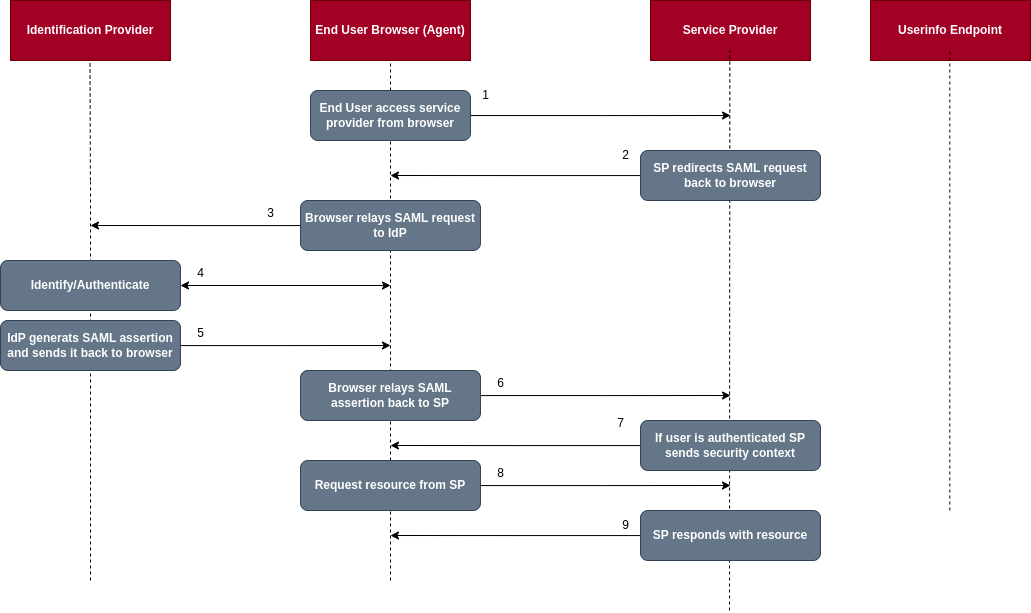
\includegraphics[width=\columnwidth]{saml-flow} 
    \caption{Diagramma di flusso dell'autenticazione con SAML}
    \label{fig:saml-flow}
\end{figure}

\subsubsection{OAuth2}
\acrshort{oauth2}\cite{site:what-is-oauth} è un protocollo di autorizzazione che consente a un'applicazione di accedere alle risorse di un utente senza richiedere le credenziali dell'utente - e, di conseguenza, senza memorizzarle - nato per assicurare l'accesso sicuro e controllato ai dati di un utente da parte di applicazioni di terze parti.

Funziona attraverso una serie di flussi di autorizzazione, in cui l'utente concede l'autorizzazione all'applicazione per accedere alle sue risorse. L'applicazione, a sua volta, ottiene un token di accesso che può essere utilizzato per accedere alle risorse dell'utente (\autoref{fig:oauth-flow-img}).

Il protocollo \acrshort{oauth2} è utilizzato da molte grandi piattaforme online come Google, Facebook e Twitter ed è diventato, di fatto, uno standard nei servizi cloud, nei social network, nei servizi di pagamento online e in molti altri contesti.
\begin{figure}[H] 
    \centering 
    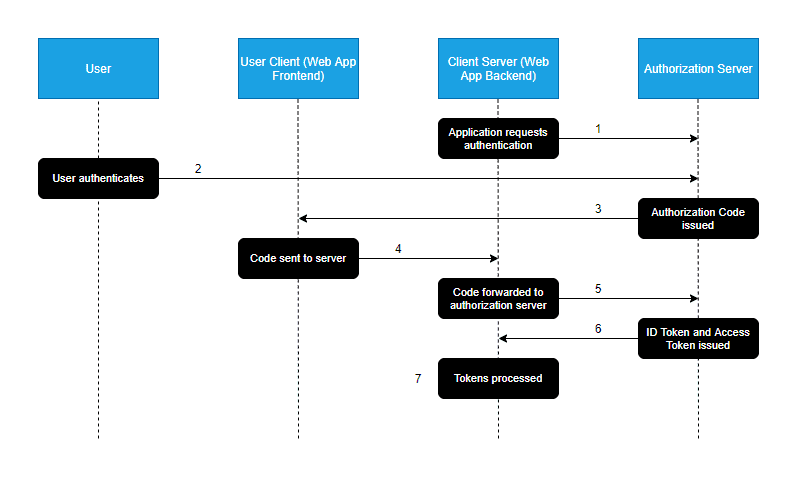
\includegraphics[width=\columnwidth]{oauth2-flow} 
    \caption{Diagramma di flusso dell'autorizzazione con OAuth2}
    \label{fig:oauth-flow-img}
\end{figure}

\subsubsection{OpenID Connect}
\acrshort{oidc}\cite{site:oidc} è un protocollo di autenticazione basato su \acrshort{oauth2}, utilizzato per l'autenticazione degli utenti in applicazioni web e mobile. Progettato per risolvere il problema dell'autenticazione sicura e decentralizzata in applicazioni di terze parti, consente agli utenti di utilizzare l'\acrshort{sso} per accedere a diverse applicazioni, senza, quindi, dover creare un nuovo account per ogni applicazione, bensì delegando l'autenticazione ad un provider esterno (OpenID Provider).

\acrshort{oidc} fornisce un framework standard per l'autenticazione basata su JSON Web Tokens (JWT), in cui l'utente viene autenticato una sola volta e poi viene rilasciato un token di accesso contenente le informazioni di base dell'utente, come l'identificatore univoco, il nome e l'e-mail, che può essere utilizzato per accedere alle risorse protette (\autoref{fig:oidc-flow-img}).

Questo protocollo è stato adottato da molte grandi piattaforme online, tra cui Google, Microsoft e Amazon ed è anche supportato da molte librerie di sviluppo, caratteristica che lo rende semplice da implementare per gli sviluppatori.
\begin{figure}[H] 
    \centering 
    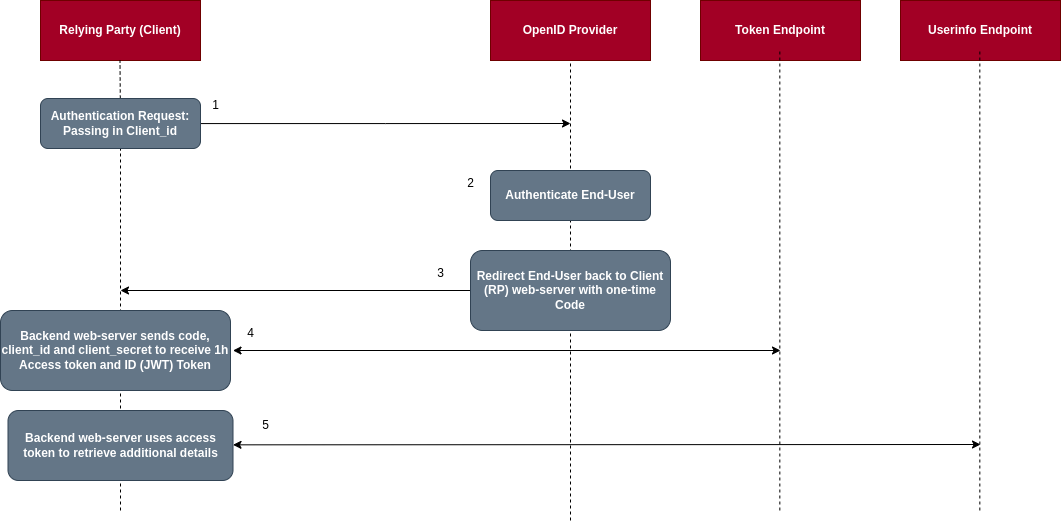
\includegraphics[width=\columnwidth]{oidc-flow} 
    \caption{Diagramma di flusso dell'autenticazione con OIDC}
    \label{fig:oidc-flow-img}
\end{figure}

\subsection{Linux Pluggable Authentication Modules}
Linux \acrshort{pam} (Pluggable Authentication Modules) è un framework di autenticazione per i sistemi operativi Linux e UNIX che consente di configurare diversi metodi di autenticazione, come quella tramite password, a due fattori, basata su token, biometrica, ecc.

Utilizzato in una vasta gamma di applicazioni e servizi, tra cui il sistema di login del sistema operativo ed il server \acrshort{ssh}, il framework di \acrshort{pam} è composto da una serie di moduli, ognuno dei quali implementa una particolare funzionalità di autenticazione. I moduli \acrshort{pam} sono progettati per essere "pluggable", ovvero possono essere facilmente sostituiti o aggiunti senza dover modificare il codice sorgente del sistema operativo.

L'architettura modulare di \acrshort{pam} consente di creare una catena di moduli, in cui ciascuno dei quali può verificare una parte dell'identità dell'utente. Ad esempio, un modulo può verificare la password dell'utente, mentre un altro può verificare il certificato del client. Se uno qualsiasi dei moduli nella catena fallisce, l'intero processo di autenticazione viene interrotto. Inoltre, è possibile sviluppare dei moduli personalizzati ed integrarli nelle diverse funzioni che richiedono \acrshort{pam}.

\section{Self-Sovereign Identity}

La \acrfull{ssi}\cite{site:ssi} è un nuovo approccio alla gestione delle identità digitali che consente agli utenti di possedere, controllare e condividere le proprie informazioni di identità in modo sicuro e privato. A differenza dei sistemi di identità tradizionali, in cui le informazioni di identità sono conservate in modo centralizzato da terze parti, l'\acrshort{ssi} consente agli utenti di essere i proprietari esclusivi dei propri dati di identità digitali.

L'\acrshort{ssi} si basa sulla tecnologia blockchain, che consente di creare registri distribuiti di informazioni sicure e immutabili. In tal modo, le informazioni di identità degli utenti vengono conservate in modo decentralizzato e sicuro, senza la necessità di un'autorità centralizzata di controllo.

Per utilizzare l'\acrshort{ssi}, gli utenti creano un'identità digitale che include le informazioni di identità necessarie, come nome, indirizzo e informazioni di contatto. Questa identità digitale viene conservata sulla blockchain e protetta da una chiave privata unica, che solo l'utente possiede.

Gli utenti possono utilizzare la propria identità digitale \acrshort{ssi} per accedere a servizi online e condividere le proprie informazioni di identità solo con le parti che desiderano. Questo viene fatto attraverso l'utilizzo di un protocollo di scambio di informazioni sicuro e decentralizzato, chiamato \acrfull{did}.

L'\acrshort{ssi} offre numerosi vantaggi, tra cui un maggiore controllo e privacy per gli utenti rispetto ai sistemi di identità tradizionali, una maggiore sicurezza attraverso l'utilizzo della tecnologia blockchain e una maggiore efficienza nella gestione delle identità digitali. Tuttavia, è ancora una tecnologia emergente e richiede una maggiore adozione e sviluppo per diventare un approccio mainstream alla gestione delle identità digitali.

\section{Tecnologie utilizzate}

Durante il periodo di stage ho avuto modo di utilizzare tecnologie per me nuove, oltre che approfondire la conoscenza di altre. Nelle sezioni seguenti sono illustrate tali tecnologie e strumenti.

\subsection{FreeIPA}
FreeIPA\cite{site:freeipa-website} (\autoref{fig:logo-freeipa}) è una soluzione open-source gratuita (GNU General Public License) di gestione dell'identità e dell'accesso per ambienti di rete basati su Linux/UNIX, originariamente sviluppato dalla comunità Fedora ed ora supportato da diverse organizzazioni, tra cui Red Hat e la FreeIPA Foundation. Consiste in un insieme di servizi integrati, che consentono di centralizzare l'autenticazione, l'autorizzazione e la gestione degli utenti e delle risorse in un'organizzazione.




FreeIPA è progettato per semplificare la gestione dell'identità e dell'accesso in ambienti di rete complessi, con molti utenti e computer. Consente agli amministratori di gestire facilmente l'accesso degli utenti a risorse e applicazioni, di delegare i privilegi di amministrazione e di definire ed applicare politiche di sicurezza coerenti in tutta la rete, come, ad esempio, limitare l'accesso alle risorse in base al ruolo dell'utente. Per fare ciò, mette a disposizione, oltre che agli strumenti della \acrshort{cli}, un'interfaccia utente web intuitiva per la gestione degli utenti, dei gruppi e delle risorse della rete. Inoltre, FreeIPA è altamente scalabile e può essere distribuito su più server per gestire grandi reti.

Per l'autenticazione degli utenti, FreeIPA utilizza il protocollo Kerberos: gli utenti possono accedere alle risorse della rete utilizzando le loro credenziali Kerberos, senza dover inserire le password ogni volta.
Per archiviare e gestire le informazioni sugli utenti, i gruppi e le risorse della rete, invece, utilizza il server di directory open-source 389 Directory Server, il quale offre funzionalità avanzate di ricerca, replica e sincronizzazione.

FreeIPA supporta l'autenticazione \acrshort{sso} tramite i protocolli \acrfull{saml} (Security Assertion Markup Language) e OICD: ciò significa che gli utenti possono accedere a più applicazioni utilizzando le stesse credenziali di accesso.
\begin{figure}[H] 
    \centering 
    
\includegraphics[width=0.45\columnwidth]{logo-freeipa} 
    \caption{Logo di FreeIPA}
    \label{fig:logo-freeipa}
\end{figure}

\subsection{Linux Containers}
\acrfull{lxc} è l'acronimo di Linux Containers, un sistema di virtualizzazione basato sul kernel Linux che consente di eseguire più sistemi operativi isolati su una singola macchina host. A differenza della virtualizzazione completa, in cui ogni sistema operativo guest ha accesso all'intero hardware dell'host, 

Utilizza la virtualizzazione basata sui contenitori, in cui ogni sistema operativo guest condivide le risorse hardware dell'host.
La condivisione del kernel fa sì che i container siano molto leggeri e veloci e che abbiano un overhead di risorse molto basso rispetto ad altre tecnologie di virtualizzazione.

\acrshort{lxc} fornisce un'interfaccia di riga di comando per la gestione dei container, che consente di creare, avviare, fermare, eliminare e gestire i container in modo semplice ed efficiente. Inoltre, supporta la creazione di immagini di container, che possono essere utilizzate per creare nuovi container in modo rapido e semplice.
\\
Durante l'attività di stage ho utilizzato principalmente container basati su immagini \acrshort{centos}, una distribuzione Linux basata su \acrshort{rhel} particolarmente adatta all'uso in ambiente server, che offre una vasta gamma di funzionalità e strumenti per gestire un'infrastruttura IT. 

In particolare, ho utilizzato l'ultima versione di \acrshort{centos} Stream (versione 9), che, a differenza della versione standard, riceve gli aggiornamenti in tempo reale durante lo sviluppo di \acrshort{ssi}, consentendo agli utenti di testare e fornire feedback sulle nuove funzionalità e correzioni di bug in anteprima\cite{site:centos-stream}.

Un'altra differenza tra \acrshort{centos} e \acrshort{centos} Stream è la durata del supporto: \acrshort{centos} ha, storicamente, fornito un supporto a lungo termine per le versioni rilasciate; la versione Stream, al contrario, è progettata per essere una piattaforma di sviluppo in continuo aggiornamento e non offre, dunque, il supporto a lungo termine.

\subsection{Secure Shell}
Secure Shell (\acrshort{ssh}) è un protocollo di rete crittografato utilizzato per la gestione sicura di dispositivi di rete e per l'accesso remoto a sistemi informatici. Il protocollo \acrshort{ssh} fornisce un canale di comunicazione sicuro tra due dispositivi, garantendo l'integrità, la riservatezza e l'autenticità delle informazioni trasmesse.

L'autenticazione avviene attraverso l'uso di chiavi pubbliche e private: in questo metodo, un'entità che desidera accedere a un sistema remoto genera una coppia di chiavi, una pubblica e una privata; la chiave pubblica viene fornita al sistema remoto, mentre la chiave privata viene conservata dall'entità; quando l'entità si connette al sistema remoto, la chiave privata viene utilizzata per autenticare l'entità.

Inoltre, \acrshort{ssh} utilizza la crittografia per proteggere i dati trasferiti tra i dispositivi. In particolare, il protocollo utilizza la crittografia a chiave simmetrica per proteggere i dati durante la trasmissione, e la crittografia a chiave pubblica per autenticare le parti coinvolte.

\subsection{Proxmox}

Proxmox è una piattaforma di virtualizzazione open-source che combina la virtualizzazione basata su container (\acrshort{lxc}) e la virtualizzazione basata su macchine virtuali (\acrfull{kvm}) in un'unica soluzione. È progettato per consentire la creazione, la gestione e l'esecuzione di macchine virtuali e container su un unico sistema, fornendo un ambiente flessibile e scalabile per le infrastrutture IT.

Una delle caratteristiche principali di Proxmox è la sua interfaccia di gestione Web, chiamata \acrfull{pve}, che fornisce un'interfaccia grafica intuitiva per la gestione delle risorse di virtualizzazione. \acrshort{lxc} consente agli amministratori di creare, configurare e monitorare le macchine virtuali e i container, nonché di gestire l'archiviazione, la rete e altre risorse di sistema.

Proxmox offre, inoltre, funzionalità avanzate come la migrazione live delle macchine virtuali, che consente di spostare una macchina virtuale in esecuzione da un nodo all'altro senza interruzioni di servizio. Ciò offre flessibilità nella gestione delle risorse e consente di bilanciare il carico di lavoro tra i nodi di virtualizzazione.

La piattaforma è anche integrata con la gestione dell'archiviazione e della rete, consentendo la creazione e la gestione di storage e reti virtuali all'interno dell'ambiente di virtualizzazione: questo semplifica la gestione delle risorse e offre una maggiore flessibilità nella configurazione dell'infrastruttura di rete e storage.
